
\section{F3 -- Thử nghiệm hội tụ OSPF}

\subsection{Mục tiêu}

Thử nghiệm F3 nhằm đánh giá khả năng phát hiện sự cố và hội tụ
của giao thức OSPF trong AS B khi một liên kết nội bộ bị gián đoạn.
Đồng thời, thử nghiệm kiểm tra khả năng duy trì phiên iBGP
khi đường truyền vật lý giữa hai router bị mất kết nối.

Cụ thể, nhóm thực hiện vô hiệu hóa liên kết L8 giữa B1 và B3
tại interface FastEthernet1/0 của B1, sau đó quan sát quá trình
OSPF phát hiện lỗi, tính toán lại đường đi và chuyển lưu lượng
sang tuyến dự phòng thông qua B2.

\subsubsection{Phương pháp thực hiện}

Trước khi gây lỗi, ba router B1, B2 và B3 đã được cấu hình
OSPF Area 0 trên các liên kết L6, L7 và L8.
Các phiên iBGP được thiết lập theo mô hình Full Mesh,
sử dụng địa chỉ Loopback0 của từng router.

Nhóm tiến hành thử nghiệm theo các bước sau:

\begin{enumerate}
    \item Kiểm tra trạng thái OSPF Neighbor và các phiên iBGP
    bằng lệnh \texttt{show ip ospf neighbor} và
    \texttt{show ip bgp summary}.

    \item Thực hiện Ping liên tục từ Loopback0 của B3
    (\texttt{10.171.26.6}) đến Loopback0 của B1
    (\texttt{10.171.26.4}).

    \item Sử dụng Wireshark để bắt gói ICMP trên liên kết L8
    (B1--B3) và L6 (B1--B2), nhằm quan sát sự thay đổi
    đường đi của lưu lượng.

    \item Thực hiện lệnh \texttt{shutdown} trên interface
    FastEthernet1/0 của B1 để mô phỏng sự cố L8.
    Interface tương ứng trên B3 vẫn được giữ nguyên.

    \item Theo dõi thông báo OSPF, quá trình tính toán SPF
    và các gói ICMP để đánh giá khả năng hội tụ.

    \item Kiểm tra đường đi thay thế và trạng thái phiên iBGP
    sau khi mạng ổn định.
\end{enumerate}

Lệnh Ping được thực hiện trên B3:

\begin{lstlisting}
ping 10.171.26.4 source Loopback0 repeat 1000 timeout 1
\end{lstlisting}

Lệnh gây lỗi trên B1:

\begin{lstlisting}
configure terminal
interface FastEthernet1/0
 shutdown
\end{lstlisting}

Để quan sát chi tiết hoạt động của OSPF, nhóm sử dụng
các lệnh debug trên B3:

\begin{lstlisting}
debug ip ospf adj
debug ip ospf spf
\end{lstlisting}

\subsection{Kết quả kiểm thử}

\paragraph{a) Kết quả Ping và phân tích Wireshark}

Kết quả Ping từ B3 đến B1 ghi nhận 994/1000 gói ICMP
thành công và 6 gói bị mất, tương ứng tỷ lệ thành công
99,4\%.

Trong quá trình bắt gói bằng Wireshark, nhóm ghi nhận:

\begin{itemize}
    \item Gói ICMP Echo Reply cuối cùng trên L8 xuất hiện
    lúc \texttt{22:03:16.415323}.
    
    \item Các gói ICMP Echo Request tiếp theo trên L8
    không nhận được phản hồi trong bản ghi bắt gói.

    \item Gói ICMP Echo Reply đầu tiên trên L6 sau khi
    chuyển đường xuất hiện lúc \texttt{22:03:22.457374}.
\end{itemize}

Khoảng thời gian giữa hai phản hồi ICMP được xác định:

\begin{equation}
\begin{aligned}
T_{\text{ICMP}}
&= 22{:}03{:}22.457374
 - 22{:}03{:}16.415323 \\
&= \boxed{6.042051\ \text{s}}
\end{aligned}
\end{equation}

Giá trị trên phản ánh khoảng thời gian giữa hai phản hồi
ICMP được quan sát trên hai liên kết, không phải thời gian
hội tụ OSPF chính xác tính từ thời điểm xảy ra lỗi.

% Thay đường dẫn bằng ảnh Wireshark L8 của nhóm.
\begin{figure}[H]
    \centering
    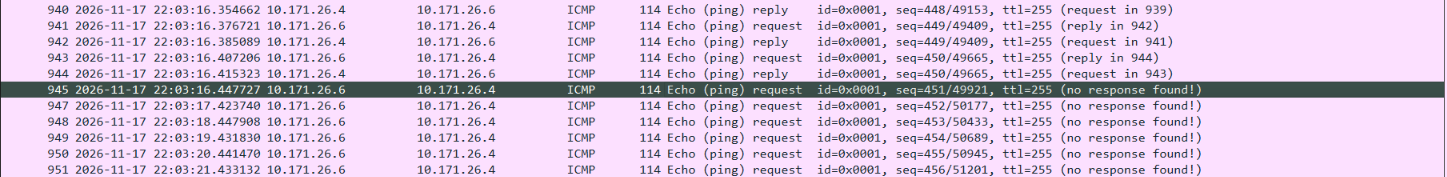
\includegraphics[width=0.95\textwidth]
    {images/testing/F3/wireshark_L8.png}
    \caption{Các gói ICMP cuối cùng trên liên kết L8 trước
    khi lưu lượng bị gián đoạn}
    \label{fig:f3-l8}
\end{figure}

% Thay đường dẫn bằng ảnh Wireshark L6 của nhóm.
\begin{figure}[H]
    \centering
    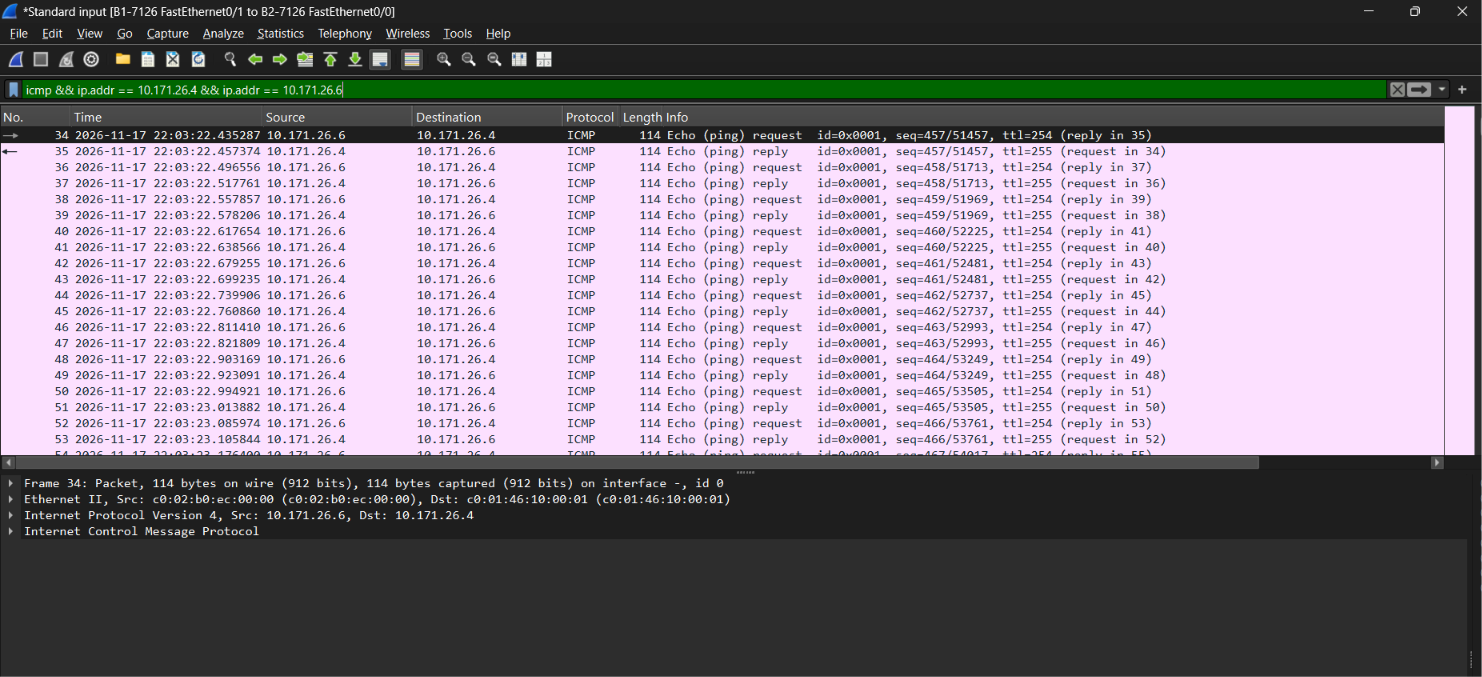
\includegraphics[width=0.95\textwidth]
    {images/testing/F3/wireshark_L6.png}
    \caption{Lưu lượng ICMP được chuyển sang liên kết L6
    sau khi OSPF tìm được đường dự phòng}
    \label{fig:f3-l6}
\end{figure}

\paragraph{b) Quá trình phát hiện lỗi và tính toán SPF}

Thông qua kết quả debug trên B3, nhóm ghi nhận các mốc
thời gian trong quá trình OSPF xử lý sự cố như
Bảng~\ref{tab:f3-spf}.

\begin{table}[H]
\centering
\caption{Các mốc thời gian xử lý OSPF trên router B3}
\label{tab:f3-spf}
\renewcommand{\arraystretch}{1.3}
\begin{tabular}{|p{8.5cm}|p{3.5cm}|}
\hline
\textbf{Sự kiện} & \textbf{Thời điểm} \\ \hline
Phát hiện OSPF Neighbor B1 DOWN
& 00:38:53.807 \\ \hline
Lên lịch thực hiện SPF
& 00:38:54.315 \\ \hline
Bắt đầu chạy thuật toán SPF
& 00:38:59.319 \\ \hline
Tính được route mới đến Loopback0 của B1
& 00:38:59.327 \\ \hline
Mốc xử lý SPF cuối cùng quan sát được
& 00:38:59.331 \\ \hline
\end{tabular}
\end{table}

Tại thời điểm \texttt{00:38:53.807}, B3 ghi nhận
OSPF Neighbor B1 chuyển từ trạng thái FULL sang DOWN
do Dead Timer hết hạn:

\begin{lstlisting}
%OSPF-5-ADJCHG: Process 1,
Nbr 10.171.26.4 on FastEthernet0/1
from FULL to DOWN,
Neighbor Down: Dead timer expired
\end{lstlisting}

Sau khi phát hiện thay đổi trạng thái Neighbor,
OSPF lên lịch chạy SPF và bắt đầu tính toán lại
đường đi tại thời điểm \texttt{00:38:59.319}.

Khoảng thời gian từ lúc phát hiện Neighbor DOWN
đến khi tính được route thay thế tới B1 là:

\begin{equation}
\begin{aligned}
T_{\text{route}}
&= 59.327 - 53.807 \\
&= \boxed{5.520\ \text{s}}
\end{aligned}
\end{equation}

Trong đó, thời gian từ lúc bắt đầu chạy SPF đến khi
tính được route tới B1 là:

\begin{equation}
T_{\text{SPF-route}}
= 59.327 - 59.319
= \boxed{0.008\ \text{s}}
\end{equation}

Như vậy, OSPF mất khoảng 5,520 giây từ khi B3
phát hiện Neighbor DOWN đến khi ghi nhận route
thay thế tới B1 trong log debug.

Khoảng thời gian này chưa bao gồm thời gian chờ
Dead Timer trước khi B3 phát hiện sự cố, cũng như
độ trễ cập nhật bảng chuyển tiếp sau khi tính toán route.

% Thay đường dẫn bằng ảnh log phát hiện Neighbor DOWN.
\begin{figure}[H]
    \centering
    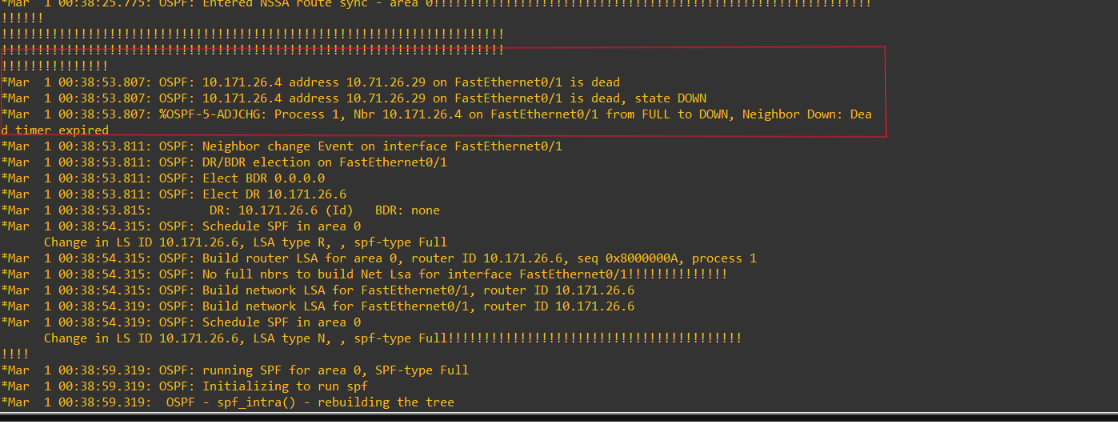
\includegraphics[width=0.95\textwidth]
    {images/testing/F3/ospf_neighbor_down.png}
    \caption{B3 phát hiện OSPF Neighbor B1 chuyển
    từ FULL sang DOWN và lên lịch chạy SPF}
    \label{fig:f3-neighbor-down}
\end{figure}

\paragraph{c) Kết quả chuyển sang đường dự phòng}

Kết quả debug SPF trên B3 ghi nhận tuyến mới đến
Loopback0 của B1:

\begin{lstlisting}
OSPF: Added Network Route to 10.171.26.4
Mask /32, Metric: 21,
Next Hop: 10.71.26.25
\end{lstlisting}

Trong đó, địa chỉ \texttt{10.71.26.25} là địa chỉ
interface của B2 trên liên kết L7.

Điều này cho thấy B3 đã tính toán được đường đi
thay thế:

\begin{center}
\textbf{B3 $\longrightarrow$ B2 $\longrightarrow$ B1}
\end{center}

Thay vì sử dụng trực tiếp liên kết L8, lưu lượng
được chuyển qua L7 và L6 để tiếp tục đến B1.

Kết quả bắt gói Wireshark trên L6 cũng ghi nhận
ICMP Echo Request và Echo Reply của luồng Ping
giữa hai địa chỉ Loopback0, xác nhận tuyến dự phòng
đã được sử dụng thành công.

% Thay đường dẫn bằng ảnh log Added Network Route.
\begin{figure}[H]
    \centering
    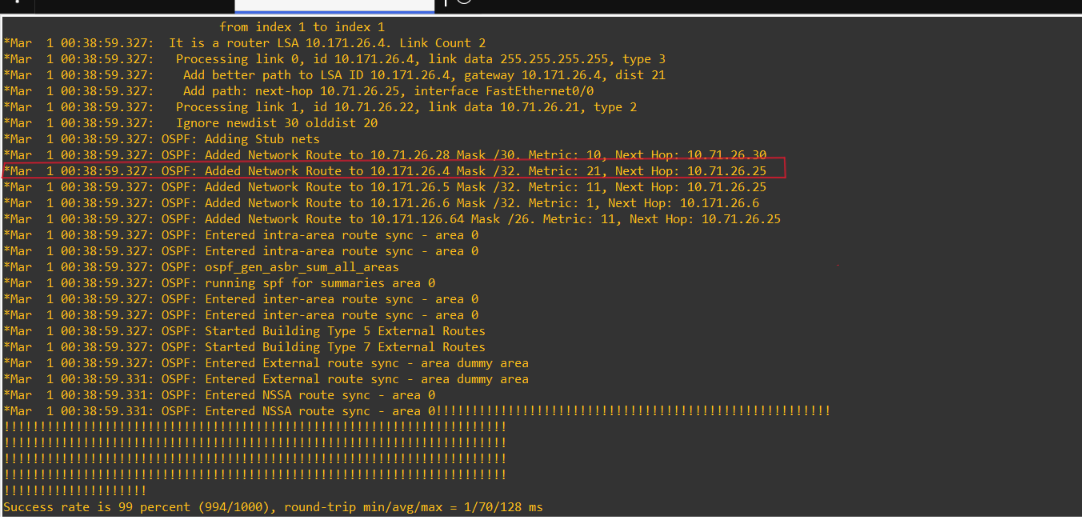
\includegraphics[width=0.95\textwidth]
    {images/testing/F3/ospf_spf_route.png}
    \caption{Kết quả tính toán SPF và lựa chọn
    next hop B2 cho tuyến đến Loopback0 của B1}
    \label{fig:f3-route}
\end{figure}



\paragraph{d) Kiểm tra khả năng duy trì phiên iBGP}

Để đánh giá ảnh hưởng của sự cố L8 đến phiên iBGP,
nhóm tiến hành kiểm tra trạng thái BGP trên cùng router
B3 trước và sau khi thực hiện shutdown liên kết L8
tại B1.

Lệnh kiểm tra được sử dụng:

\begin{verbatim}
show ip bgp summary
\end{verbatim}

Kết quả được ghi nhận trong
Bảng~\ref{tab:f3-ibgp-comparison}.

\begin{table}[H]
    \centering
    \caption{So sánh trạng thái iBGP trên B3 trước và sau sự cố}
    \label{tab:f3-ibgp-comparison}
    \renewcommand{\arraystretch}{1.3}
    \begin{tabular}{|l|c|c|}
        \hline
        \textbf{Thông số} &
        \textbf{Trước shutdown} &
        \textbf{Sau shutdown} \\
        \hline
        Neighbor & 10.171.26.4 & 10.171.26.4 \\
        \hline
        Up/Down & 00:05:47 & 00:06:42 \\
        \hline
        State/PfxRcd & 1 & 1 \\
        \hline
        MsgRcvd & 9 & 10 \\
        \hline
        MsgSent & 11 & 12 \\
        \hline
    \end{tabular}
\end{table}

\textbf{Trước khi gây lỗi:}

Phiên iBGP giữa B3 và B1 đang ở trạng thái
Established, với thời gian hoạt động là
\texttt{00:05:47}.

\begin{figure}[H]
    \centering
    \includegraphics[width=0.95\textwidth]
    {images/testing/F3/ibgp_before.png}
    \caption{Trạng thái phiên iBGP trên B3
    trước khi shutdown liên kết L8}
    \label{fig:f3-ibgp-before}
\end{figure}

\textbf{Sau khi gây lỗi:}

Kết quả kiểm tra cho thấy phiên iBGP với B1
vẫn ở trạng thái Established, với thời gian
Up/Down tăng lên \texttt{00:06:42}.

\begin{figure}[H]
    \centering
    \includegraphics[width=0.95\textwidth]
    {images/testing/F3/ibgp_after.png}
    \caption{Trạng thái phiên iBGP trên B3
    sau khi shutdown liên kết L8}
    \label{fig:f3-ibgp-after}
\end{figure}

\textbf{Nhận xét:}

Giá trị Up/Down tăng từ 00:05:47 lên 00:06:42,
tương ứng 55 giây, và không có dấu hiệu
bị đặt lại trong hai lần quan sát.

Đồng thời, số bản tin BGP nhận được tăng từ
9 lên 10 và số bản tin gửi đi tăng từ 11 lên 12.
Cột State/PfxRcd tiếp tục hiển thị giá trị 1,
cho thấy phiên iBGP đang ở trạng thái Established.

Kết quả này cho thấy phiên iBGP giữa B1 và B3
được duy trì tại các thời điểm kiểm tra,
phù hợp với cơ chế sử dụng Loopback0 để
thiết lập phiên BGP và khả năng chuyển đường
dự phòng của OSPF.

